% Imported from LaTeX_and_pdfs/DGDT_dump.tex; see provenance.json.
\part{Connections}


\section{Connections of Vector Bundles}

Morita (2001) \cite{dgdt:Mori2001}

\begin{definition}[Connection in a vector bundle]
	\textbf{connection in a vector bundle} $\pi : E \to M$ over $C^{\infty}$ manifold $M$, is a bilinear map
	\[
	\nabla : \mathfrak{X}(M) \times \Gamma(E) \to \Gamma(E)
	\]
	satisfying
	\begin{enumerate}
		\item[(i)] $\nabla_{fX} s = f\nabla_X s$
		\item[(ii)] $\nabla_X(fs) = f\nabla_Xs + (Xf)s$ where $f\in C^{\infty}(M)$, $X \in \mathfrak{X}(M)$, $s\in \Gamma(E)$
	\end{enumerate}
$\nabla_Xs$ is covariant derivative of $s$ relative to $X$ (for Morita (2001)\cite{dgdt:Mori2001})

Alternatively, Jost (2017) \cite{dgdt:Jost2017} defines in the following way: \\

Let vector bundle $(E, \pi, M)$, where differentiable manifold $M$, vector bundle $E$ over $M$; a covariant derivative or (linear) connection is map
\begin{equation}
	D:\Gamma(E) \to \Gamma(E) \otimes \Gamma(T^*M) \equiv \Gamma(E) \otimes \mathfrak{X}(M)
\end{equation}
(we may also consider $D$ as map $D: \mathfrak{X}(M) \otimes \Gamma(E) \to \Gamma(E)$, with $s \in \Gamma(E), X \in \mathfrak{X}(M), DX(s) \equiv D_X s$) s.t.

\begin{enumerate}
	\item $D$ is tensorial in $\mathfrak{X}(M)$, 
	\begin{equation}
		\begin{gathered}
			D_{X +Y} s = D_X s + D_Y s \quad \, \forall \, X,Y \in T_xM, \, s\in \Gamma(E) \\
			D_{fX} s = fD_X s \quad \, \forall \, f \in C^{\infty}(M, \mathbb{R}), \, X \in \Gamma(TM)
		\end{gathered}
	\end{equation}
\item $D$ is $\mathbb{R}$-linear in $s$, 
\begin{equation}
	D_X(s+t ) = D_X s + D_X t \quad \, \forall \, X \in T_xM , \, s,t \in \Gamma(E) 
\end{equation}
and product rule
\begin{equation}
	D_X(fs) = X(f) \cdot s + fD_X(s) \quad \, \forall \, f \in C^{\infty} (M, \mathbb{R})
\end{equation}
\end{enumerate}

\end{definition} 

\underline{Claim}: \emph{Any vector bundle admits a connection}.

e.g. product bundle $M\times \mathbb{R}^n$. Let $x_1, \dots , x_n$ be canonical coordinates in $\mathbb{R}^n$. Take frame field $(s_1, \dots, s_n)$, where $s_i(p) = \frac{\partial}{\partial x^i}$. Set $\nabla_X s_i =0 $ ($i=1,\dots , m$) \quad \, $\forall \, $ vector space $X$, \\
$\forall \, s = \sum_i a_i s_i, \, \forall X \in \mathfrak{X}(M)$, set 
\[
\nabla_X s = \sum_{i=1}^n (Xa_i) s_i
\]
For this connection $\nabla_Xs$ is the partial derivative in direction of $X$ if $s$ is considered $\mathbb{R}^n$-valued function on $M$. Call it \textbf{trivial connection} in product bundle.

Indeed,
\[
\begin{gathered}
	\nabla_X s = \nabla_{ X^i \frac{\partial}{\partial x^i}} \left( s^m \frac{\partial}{\partial x^m} \right) = X^i \nabla_{ \frac{\partial}{\partial x^i} } \left( s^m \frac{\partial}{\partial x^m} \right) = X^i \left( \nabla_{ \frac{\partial}{\partial x^i} } s^m \right) \frac{\partial}{\partial x^m} + X^i s^m \nabla_{ \frac{\partial}{\partial x^i} } \frac{\partial}{\partial x^m} = \\	
		= X^i \left( \frac{\partial}{\partial x^i} s^m \right) \frac{\partial}{\partial x^m} + X^i s^m \Gamma^q_{ \, \, mi} \frac{\partial}{\partial x^q} = X^i \frac{ \partial s^m}{ \partial x^i} \frac{\partial }{ \partial x^m } + 0 
\end{gathered}
\]
if $\Gamma^q_{ \, \, mi} =0$ at a chosen point $p$.

For arbitrary vector bundle $\pi : E \to M$, take locally finite open covering $\lbrace U_{\alpha} \rbrace_{\alpha \in A}$ s.t. $\pi^{-1}(U_{\alpha})$ trivial. Denote $\nabla^{\alpha} $ trivial connection $\forall \, \pi^{-1}(U_{\alpha})$. Let $\lbrace f_{\alpha} \rbrace$ be a partition of unity for covering $U_{\alpha}$, define 
	\[
	\nabla_X s := \sum_{\alpha} f_{\alpha} \nabla_X^{\alpha} s
	\]

Verify this defines connection in $E$:
\[
\begin{gathered}
\nabla_X(gs) = \sum_{\alpha} f_{\alpha} \nabla^{\alpha}_X(gs) = \sum_{\alpha} f_{\alpha} \left[ X^i \left( \frac{\partial g}{\partial x^i} \right) s + X^i g \frac{\partial s^m}{\partial x^i} \frac{\partial}{\partial x^m} \right] = \\
= g \sum_{\alpha} f_{\alpha} \nabla_X^{\alpha} s + \sum_{\alpha} f_{\alpha} (Xg) s
\end{gathered}
\]

\begin{proposition}[5.18 Morita (2001)\cite{dgdt:Mori2001}]
Let $\nabla_i$ ($1 \leq i \leq k$) be $k$ connections in a given vector bundle. Then $\forall \, $ linear combination $\sum_{i=1}^k t_i \nabla_i$, where $t_1 + \dots + t_k =1$ is a connection.	
\end{proposition} 

\begin{proof}
	TODO: Ex. 5.5
\end{proof} 

\subsection{Directional derivatives of tensor fields; Connections on a tensor product}

cf. Schuller (2015) \cite{dgdt:Schul2015}, \href{https://youtu.be/nEaiZBbCVtI}{Lecture 7: Connections (International Winter School on Gravity and Light 2015))}.

\begin{definition}[Connection on tensor fields]
	A \textbf{connection} $\nabla$ or smooth manifolds $(M, \mathcal{O}, \mathcal{A})$ is a map $\nabla : \mathfrak{X}(M) \times \Gamma(TM^p \otimes T^*M^q) \to \Gamma(TM^p \otimes T^*M^q)$, \\
	where $\binom{p}{q}$ tensor-field section $\equiv \Gamma (TM^p \otimes T^*M^q)$
	
	\begin{enumerate}
		\item $\nabla_X f = Xf \quad \, \forall \, f \in C^{\infty}(M)$ 
		\item $\nabla_X(T+S) = \nabla_XT  + \nabla_XS$ 
		\item $\nabla_X(T(\omega, Y)) = (\nabla_XT)(\omega, Y) + T(\nabla_X \omega, Y) + T(\omega, \nabla_X Y)$, where $T(\omega, Y) \in C^{\infty}(M)$ \\
		
		This is written for a $(1, 1)$ tensor field $T$, but is analogously true $\forall \, (p, q)$ tensor field. 
		\item $\nabla_{fX + Z} T = f\nabla_X T + \nabla_Z Y$, where $f\in C^{\infty}(M)$ \\
		
		Consider also product rule $\nabla_X(fT) = X(f) T + f\nabla_XT \quad \, \forall \, f \in C^{\infty}(M, \mathbb{R})$
	\end{enumerate}

A manifold with connection is a quadruple $(M, \mathcal{O}, \mathcal{A}, \nabla)$
\end{definition}

Consider 
\[
\begin{gathered}
	\begin{aligned}
		\nabla_X Y & = \nabla_{X^i \frac{ \partial }{ \partial x^i} } \left(Y^m \frac{\partial }{ \partial x^m } \right) = X^i \nabla_{\frac{\partial}{\partial x^i} } \left( Y^m \frac{ \partial }{\partial x^m} \right) = X^i \left[ \left( \nabla_{\frac{ \partial }{ \partial x^i} } Y^m \right) \frac{\partial }{ \partial x^m} + Y^m \nabla_{\frac{\partial }{ \partial x^i} } \frac{\partial}{ \partial x^m} \right] = \\
		& = X^i \frac{\partial Y^m}{\partial x^i} \frac{\partial }{\partial x^m } + X^i Y^m  \Gamma^q_{ \, mi } \frac{\partial}{\partial x^q}
	\end{aligned}
\end{gathered}\]

so then

\begin{definition}[Connection coefficient functions, i.e. Christoffel Symbols]
	\begin{equation}
		\begin{aligned}
			\Gamma^i_{\, jk} & : \mathcal{U} \to \mathbb{R} \\
			& p \mapsto ( dx^i \left( \nabla_{\frac{\partial}{\partial x^k} } \frac{\partial }{ \partial x^j} \right) )(p)
		\end{aligned}
	\end{equation}
\end{definition}

Now since
\[
\begin{gathered}
	\begin{gathered}
		\nabla_{\frac{\partial}{\partial x^m} } \left( dx^i \left( \frac{ \partial }{ \partial x^j} \right) \right) = \nabla_{\frac{\partial}{\partial x^m} } (\delta^i_{\, \, j} ) = 0 \text{ so } \\
		\nabla_{\frac{\partial}{\partial x^m} } \left( dx^i \left( \frac{ \partial }{ \partial x^j} \right) \right) = \left( \nabla_{\frac{\partial}{\partial x^m} } dx^i \right) \left( \frac{\partial }{ \partial x^j} \right) + dx^i \left( \nabla_{\frac{\partial}{\partial x^m} } \frac{\partial }{ \partial x^j} \right) = \left( \nabla_{\frac{\partial}{\partial x^m} } dx^i \right) \left( \frac{\partial }{ \partial x^j} \right) + dx^i \Gamma^q_{\, jm} \frac{ \partial }{ \partial x^q} = 0 \\
		\Longrightarrow \boxed{ \left( \nabla_{\frac{\partial}{\partial x^m} } dx^i \right) \left( \frac{\partial }{ \partial x^j} \right) = -\Gamma^i_{\, jm} } \text{ since } \\
		dx^i \Gamma^q_{\,  jm} \frac{\partial }{ \partial x^q} = \Gamma^q_{\, jm} dx^i \left( \frac{\partial }{ \partial x^q} \right) = \Gamma^q_{\, jm} \delta^i_{\, q} = \Gamma^i_{\, jm}
	\end{gathered}
\end{gathered}\]

	\subsubsection{Change of $\Gamma$'s under change of chart}

cf. \href{https://youtu.be/nEaiZBbCVtI?t=4130}{1:08:50 3. Change of $\Gamma$'s under change of chart}, Schuller (2015) \cite{dgdt:Schul2015}

$(U,x)$, $(V,y) \in \mathcal{A}$ and $U \cap V \neq \emptyset$

\[
\Gamma^i_{jk}(y) := dy^i \left( \nabla_{ \frac{ \partial}{ \partial y^k} } \frac{ \partial }{ \partial y^j} \right) = \frac{ \partial y^i}{ \partial x^q }dx^q \left( \nabla_{\frac{ \partial x^p}{ \partial y^k}  \frac{ \partial }{ \partial x^p} } \frac{ \partial x^s}{ \partial y^j} \frac{ \partial }{ \partial x^s } \right)
\]
because, \\
since $y^i$ is a function, i.e. \\
$y^i = y^i(x)$, and $d$ acts on a function, then $dy^i = dy^i(x) = \frac{ \partial y^i}{\partial x^q} dx^q$, and since
\[
\frac{\partial f(y) }{ \partial y^k} = \frac{\partial f(x(y)) }{ \partial y^k} = \frac{ \partial x^p }{ \partial y^k} \frac{ \partial f(x) }{ \partial x^p} \text{ so } \frac{ \partial }{ \partial y^k} = \frac{\partial x^p}{ \partial y^k} \frac{\partial}{ \partial x^p} \text{ by chain rule }
\]

Note $\nabla_{fX}$ is $C^{\infty}$-linear for $fX$

covector $dy^i$ is $C^{\infty}$-linear in its argument
\[
\begin{aligned}
	\Longrightarrow \Gamma_{jk}^i(y) & = \frac{ \partial y^i}{ \partial x^q} dx^q \left( \frac{ \partial x^p}{ \partial y^k} \left[ \left( \nabla_{ \frac{ \partial }{ \partial x^p} } \frac{ \partial x^s}{ \partial y^j} \right) \frac{ \partial }{ \partial x^s} + \frac{ \partial x^s}{ \partial y^j} \left( \nabla_{ \frac{ \partial }{ \partial x^p } } \frac{ \partial }{ \partial x^s } \right)  \right] \right) = \\
	& = \frac{ \partial y^i}{ \partial x^q} \underbrace{\frac{ \partial x^p }{ \partial y^k} \frac{ \partial }{ \partial x^p }}_{\frac{\partial}{\partial y^k} } \frac{ \partial x^s}{ \partial y^j } \delta^q_{ \, \, s} + \frac{ \partial y^i}{ \partial x^q} \frac{ \partial x^p }{ \partial y^k} \frac{ \partial x^s}{ \partial y^j} \Gamma^q_{sp}(x)
\end{aligned}
\]


In summary (Schuller says to commit this to memory):
\begin{equation}\label{dgdt:Eq:ChangeofGamma}
	\boxed{ \Gamma^i_{jk}(y) = \frac{ \partial y^i}{ \partial x^q} \frac{ \partial^2 x^q}{ \partial y^j \partial y^k} + \frac{ \partial y^i}{ \partial x^q } \frac{ \partial x^s }{ \partial y^j} \frac{ \partial x^p }{ \partial y^k} \Gamma^q_{sp}(x) }
\end{equation}
Eq. (\ref{dgdt:Eq:ChangeofGamma}) is the change of connection coefficient function under the change of chart $(U\cap V,x) \to (U\cap V,y)$ Notice especially the second-order partial derivative term: for any linear transformation, this term will "not be felt" (i.e. will be zero), but otherwise for a nonlinear transformation of coordinates, you'll "feel it."


\subsubsection{Normal Coordinates}

Let $p \in M$ of $(M, \mathcal{O}, \mathcal{A}, \nabla)$

Then one can construct a chart $(U,x)$ with $p\in U$ such that 
\begin{equation}\label{dgdt:Eq:SymmetricPartZeroForNormalCoordinates}
\begin{gathered}
	\Gamma(x)^i_{\,\, (jk)}(p) = 0
\end{gathered} 
\end{equation}
\emph{at} the point $p$. \textbf{Not} necessarily in any neighborhood. Note the $(jk)$ subscript, meaning the symmetric part vanishes, i.e. equals zero. So Eq. \ref{dgdt:Eq:SymmetricPartZeroForNormalCoordinates} says we can choose a coordinate system such that at a point the symmetric part of the Christoffel Symbol is zero.

Recall the definition of symmetric and antisymmetric parts of some tensor $T$. Define the symmetric and antisymmetric parts, respectively:
\[
\begin{aligned}
	& T_{(ab)} = \frac{1}{2} ( T_{ab} + T_{ba}) \\
	& T_{[ab]} = \frac{1}{2} ( T_{ab} - T_{ba}) \\
\end{aligned}
\]

\begin{proof}
	Let $(V,y)$ be any chart (with) $p\in V$.
	
	Thus, in general: $\Gamma(y)^i_{\,\, jk} \neq 0$
	
	Then consider a new chart $(U, x)$ to which one transits by virtue of 
	\[
	\begin{gathered}
		(x\circ y^{-1})^{i}(\alpha^1, \dots, \alpha^d) := \alpha^i - \frac{1}{2} \Gamma(y)^i_{\,\, (jk)}(p) \alpha^j \alpha^k 
	\end{gathered}
	\]
	for $p = x^{-1}(\alpha^1, \dots , \alpha^d)$
	
	\[
	\begin{gathered}
		\begin{aligned} 
			& \left(\frac{\partial x^i}{ \partial y^j}\right)_p = \partial_j (x^i \circ y^{-1}) = \delta^i_j - \Gamma(y)^i_{\,\, mj}(p) \left. \alpha^m \right|_{\alpha = 0} = \delta^i_j \\
			& \frac{\partial x^i}{ \partial y^k \partial y^j}(p) = - \Gamma(y)^i_{ \, \, (kj)} (p)
		\end{aligned} 
	\end{gathered}
	\]
where the partial derivative acting on the second term with the Christoffel symbol is because of the following:
\[
\begin{gathered}
	\frac{\partial}{\partial y^j} \frac{1}{2} \Gamma(y)^i_{\, (lk)} (p) \alpha^l \alpha^k = \frac{\partial}{\partial \alpha^j} \frac{1}{2} \Gamma(y)^i_{\, (lk)} (p) \alpha^l \alpha^k = \frac{1}{2} \Gamma(y)^i_{\, (lk)} (p) \delta^l_{\, j} \alpha^k + \frac{1}{2} \Gamma(y)^i_{\, (lk)} (p) \alpha^l \delta^k_{\, j} = \\
	= \frac{1}{2} \Gamma(y)^i_{\, (jk)} (p)  \alpha^k + \frac{1}{2} \Gamma(y)^i_{\, (lj)} (p)  \alpha^l = \Gamma(y)^i_{\, (jm)}(p) \alpha^m
\end{gathered}
\]
where the last step is by the symmetry property of the symmetric part of $\Gamma^i_{\, jm}$, $\Gamma^i_{\, (jm)}$.

Then use Eq. (\ref{dgdt:Eq:ChangeofGamma}), the change of Christoffel symbols equation we just derived:
\[
\begin{gathered}
\Gamma^i_{jk}(y) = \frac{ \partial y^i}{ \partial x^q} \frac{ \partial^2 x^q}{ \partial y^j \partial y^k} + \frac{ \partial y^i}{ \partial x^q } \frac{ \partial x^s }{ \partial y^j} \frac{ \partial x^p }{ \partial y^k} \Gamma^q_{sp}(x)	= \frac{ \partial y^i}{ \partial x^q} \left( - \Gamma(y)^q_{ \, \, (kj)} (p) \right) + \frac{ \partial y^i}{ \partial x^q } \Gamma^q_{ \, \, jk} (x)
\end{gathered}
\]

\emph{If} $\frac{\partial y^i}{\partial x^q} = -\delta^i_{\, \, q}$ then we obtain 
\[
\begin{gathered}
	\Gamma^i_{\, \, jk} (y) = + \Gamma(y)^i_{\,\, (jk)} - \Gamma^i_{\,\, jk} (x) \text{ or  } \\
	\Gamma^i_{\, \, jk} (x) = - \Gamma^i_{\, \, jk} (y) + \Gamma^i_{\, \, (jk)} (y) = \Gamma(y)^i_{\, \, [kj]}
\end{gathered}
\]


Compare this against what Schuller (2015) \cite{dgdt:Schul2015} obtains:
	\[
	\begin{gathered}
		\begin{aligned} 
			\Longrightarrow \Gamma(x)^i_{jk}(p) & = \Gamma(y)^i_{\,\, (jk)}(p)  -  \Gamma(y)^i_{\,\, kj}(p) =  \\
			& = \Gamma(y)^i_{[jk]}(p) = T(y)^i_{\,\,jk}
		\end{aligned} 
	\end{gathered}
	\]
	
	\underline{Terminology}: $(U,x)$ is called a \textbf{normal coordinate chart} of $\nabla$ at {$\mathbf{p\in M}$}.
	
\end{proof}



cf. pp. 164, 4.1 \emph{Connections in Vector Bundles}, Jost (2017) \cite{dgdt:Jost2017}

Let $x_0 \in M$, let open neighborhood $U$ of $x_0$ s.t. $\exists$ chart for $M$, $\exists\,$ bundle chart for $E$ on $U$. Thus, $\exists$ coordinate vector fields $\frac{\partial }{ \partial x^1} , \cdots \frac{\partial }{ \partial x^d}$ and through identification
\[
\left. E \right|_U \simeq U \times \mathbb{R}^n
\]
$n = $ fiber dim. of $E$.

For \emph{a} basis of $\mathbb{R}^n$ yields basis $\mu_1 \dots \mu_n \equiv e_q \dots e_n$ of sections of $\left. E \right|_U \equiv \Gamma(\left. E \right|_U )$. Define Christoffel symbols $\Gamma^k_{\, ij}$ ($j,k =1\dots n, i =1 \dots d$) (pp. 164, Jost (2017) \cite{dgdt:Jost2017}) 

\begin{equation}
	\begin{aligned}
		D_{\frac{\partial}{\partial x^i} } \mu_j & := \Gamma^k_{\, ij} e_k \quad \, (\text{4.1.5, Jost (2017)\cite{dgdt:Jost2017}}) \\
		\equiv D_{\frac{\partial}{\partial x^j} } e_i & \Gamma^k_{\, ij} e_k \quad \, (\text{Schuller's notation})\\
	\end{aligned}
\end{equation}

\subsection{Parallel Transport}

Let $\mu \equiv s \in \Gamma(E)$, ($\mu$ is the notation of Jost (2017) \cite{dgdt:Jost2017}) locally $s(y) = a^k(y) e_k(y)$, let $c(t) =$ smooth curve in $U$. \\
Let $s(t):= s(c(t))$, to define a section of $E$ along $c$. \\
Let $X(t) = \dot{c}(t) = \dot{c}^i(t) \frac{\partial}{\partial x^i}$ \\

Then
\[
\begin{gathered}
	D_{X(t)} s(t) = D_{\dot{c}^i \frac{\partial}{\partial x^i} } s(t) = \dot{c}^i D_{ \frac{\partial }{\partial x^i}} a^k e_k = \dot{c}^i \left( \frac{ \partial a^k}{ \partial x^i} \right) e_k + \dot{c}^i a^k \Gamma^q_{\, ki} e_q = \\
	= \left( \dot{a}^k + \dot{c}^j a^i \Gamma^k_{\, ij} \right) e_k
\end{gathered}\]
where we had used chain rule:
\[
\dot{a}^k \equiv \frac{da^k}{dt} = \frac{\partial a^k}{\partial x^i} (x(t)) \frac{dc^i}{dt}
\]
So if $D_{x(t)} s(t) = 0$, we have $k=1 \dots n$ first order linear equations, solving for $a^1, \dots a^n(t)$.

So by a fundamental theorem for ordinary differential equations (ODEs), for given initial values $s(0) \in E_{c(0)}$, $\exists !$ solution to $D_{x(t)} s(t) = 0$.

\begin{definition}[Parallel transport of section of vector bundle, Def. 4.1.2, Jost (2017)\cite{dgdt:Jost2017}]
The solution set of $D_{x(t)} s(t) = 0$	 is called the parallel transport of $s(0)$ along curve $c$.
\end{definition}

Given $X \in T_xM$, let curve $c$ in $M$ with $c(0) = x$, $\dot{c}(0) = X$, $\forall \, s \in \Gamma(E)$, then
\[
D_X s := \lim_{t \to 0} \frac{ P_{c,t}(s(c(t))) - s(c(0)) }{ t}
\]
EY: This seems to be the covariant derivative.

pp. 165 Jost (2017) \cite{dgdt:Jost2017} claims that parallel transport on Riemannian manifold can obtain covariant derivative.

\begin{proof}
	Let $P_{c,t} : E_{c(t)} \to E_{c(0)} $ be identification by parallel transport along $c$.
	
	Select a basis of parallel sections $\mu_1(t), \dots \mu_n(t) \equiv e_1(t) \dots e_n(t)$ of $E$ along $c$, i.e.
	\[
	D_{\dot{c}(t) } e_j(t) = 0 \quad \, \forall \, j = 1 \dots n
	\]
	
	$\forall \,$ arbitrary section $s$ of $E$ along $c$, then 
	\[
	s(t) = a^k(t) e_k(t)
	\]
	and for $X = \dot{c}(0)$,
	\[
	\begin{gathered}
		D_X s(t) = D_X(a^k(t) e_k(t)) = D_X(a^k(t)) e_k(t) + a^k(t) D_X e_k(t) = \dot{a}^k(t) e_k(t)
	\end{gathered}
	\]
	where $D_Xe_k(t)=0$ by parallel transport.
	
	So
	\[
	\begin{gathered}
		(D_Xs) (c(0)) = \lim_{t\to 0} \frac{a^k(t) - a^k(0) }{ t} e_k(0) = \lim_{t\to 0} \frac{ P_{c,t} (s(t)) - s(0) }{t}
	\end{gathered}
	\]
\end{proof}

Consider tangent space at pt. $\psi \equiv s$ to the total space $E$ of a vector bundle $T_sE$. \\
Inside $T_sE$, there's a distinguished subspace, namely the tangent space to the fiber $E_x$ containing $s$ ($x=\pi(s)$). \\
This space is called vertical space $V_s$. \\

However, there's no distinguished "horizontal space" $H_s$ complementary to $V_s$, i.e. $T_sE = V_s \oplus H_s$. \\
If we have covariant derivative $D$, we can parallel transport $s$, $\forall\, X \in T_xM$ along curve $c(t)$ with 
\[
c(0) = x, \, \dot{c}(0) = X
\]

Thus, $\forall \, X$, we obtain a curve $s(t) $ in $E$. \\
subspace of $T_sE$ spanned by all tangent vectors to $E$ at $s$ of the form
\[
\left. \frac{d}{dt} s(t) \right|_{t=0}
\]
then is the horizontal space $H_s$.

\subsubsection{Parallelity of vector fields}

cf. Lecture 8, Schuller (2015) \cite{dgdt:Schul2015}.

Assume smooth affine manifold $(M, \mathcal{O}, \mathcal{A}, \nabla)$ with connection.

\begin{definition}[Parallely Transported]
	vector field $X$ on $M$ is \textbf{parallely transported} along smooth curve $\gamma:\mathbb{R} \to M$ if 
	\begin{equation}
		\nabla_{v_{\gamma}} X = 0
	\end{equation}
\end{definition}

\begin{definition}[Parallel]
	vector field $X$ in $M$ is \textbf{parallel} along curve $\gamma:\mathbb{R} \to M$ if $\nabla_{v_{\gamma}} = \mu \cdot X$
\end{definition}

\begin{center}
	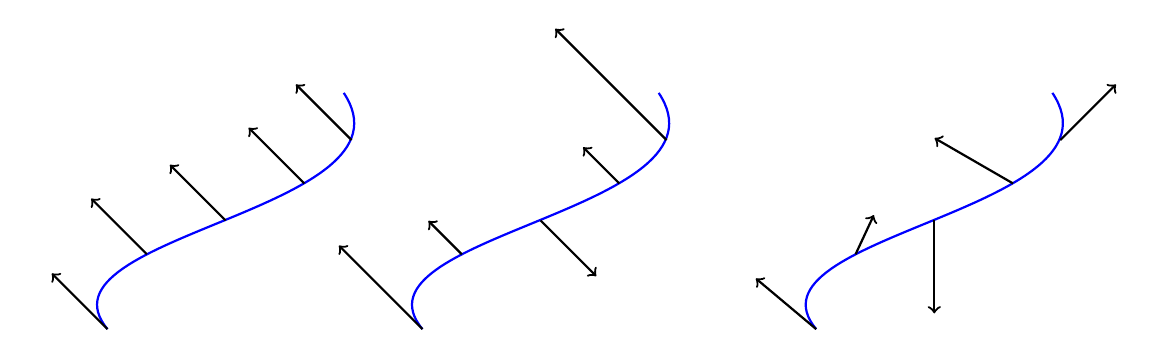
\begin{tikzpicture}
	\draw[thick, blue] (-4,0) .. controls (-5,1.2) and (0,1.5) .. (-1,3);
	\draw[thick, blue] (0,0) .. controls (-1,1.2) and (4,1.5) .. (3,3);
	\draw[thick, blue] (5,0) .. controls (4,1.2) and (9,1.5) .. (8,3);
	\draw[->, thick, rotate around={45: (-4,0)}] (-4,0) -- (-4,1);
	\draw[->, thick, rotate around={45: (-3.5,0.95)}] (-3.5,0.95) -- (-3.5,1.95);
	\draw[->, thick, rotate around={45:(-2.5,1.38)}] (-2.5,1.38) -- (-2.5,2.38);
	\draw[->, thick, rotate around={45:(-1.5,1.85)}] (-1.5,1.85) -- (-1.5,2.85);
	\draw[->, thick, rotate around={45:(-0.9,2.4)}] (-0.9,2.4) -- (-0.9,3.4);
	\draw[->, thick, rotate around={45: (0,0)}] (0,0) -- (0,1.5);
	\draw[->, thick, rotate around={45: (0.5,0.95)}] (0.5,0.95) -- (0.5,1.55);
	\draw[->, thick, rotate around={45:(1.5,1.38)}] (1.5,1.38) -- (1.5,0.38);
	\draw[->, thick, rotate around={45:(2.5,1.85)}] (2.5,1.85) -- (2.5,2.5);
	\draw[->, thick, rotate around={45:(3.1,2.4)}] (3.1,2.4) -- (3.1,4.4);
	\draw[->, thick, rotate around={50: (5,0)}] (5,0) -- (5,1);
	\draw[->, thick, rotate around={-25: (5.5,0.95)}] (5.5,0.95) -- (5.5,1.5);
	\draw[->, thick] (6.5,1.38) -- (6.5,0.2);
	\draw[->, thick, rotate around={60:(7.5,1.85)}] (7.5,1.85) -- (7.5,3);
	\draw[->, thick, rotate around={-45:(8.1,2.4)}] (8.1,2.4) -- (8.1,3.4);
	\end{tikzpicture}
\end{center}
The left drawing is a parallely transported vector field, the middle drawing is a parallel vector field. For the middle drawing, it's important that the vector field vanishes in-between points when it points "up" vs. "down" because $\mu:\mathbb{R} \to \mathbb{R}$ is smooth. The right drawing is not even parallel.

\subsubsection{Autoparallelly Transported Curves}

\begin{definition}[Autoparallely Transported]
	smooth curve $\gamma : \mathbb{R} \to M$ \textbf{autoparallely transported} if 
	\begin{equation}
		\nabla_{v_{\gamma}} v_{\gamma} = 0
	\end{equation}
\end{definition}

\begin{definition}
	smooth curve $\gamma : \mathbb{R} \to M$ is autoparallel 
	\begin{equation}
		\nabla_{v_{\gamma}} v_{\gamma} = \mu v_{\gamma}
	\end{equation}
for some smooth $\mu:\mathbb{R}\to \mathbb{R}$
\end{definition}

For autoparallel, it means we move in the straightest line. We are not talking about the shortest line because we do not have a notion of distance.

Note that the straightest line might not actually look straight when "viewed from above." That is, if we embed the manifold into a higher dimensional one, and then just look at the curve, it might be curved. For example, on a sphere, a straight line traces out a portion of a circle around the sphere. This doesn't look straight in the (higher, Euclidean) embedding, but \emph{on the surface} of the sphere, it's the straightest line.

\begin{center}
	\begin{tikzpicture} 
	\draw[thick] (-2,-2) -- (-1.5,-1.5);
	\draw[thick] (-1.4,-1.4) -- (-0.9,-0.9);
	\draw[thick] (-0.8,-0.8) -- (-0.3,-0.3);
	\draw[thick] (-0.2,-0.2) -- (0.3,0.3);
	\draw[thick] (0.4,0.4) -- (0.9,0.9);
	\draw[thick] (1,1) -- (1.5,1.5);
	\draw[thick] (2,-2) -- (2.5,-1.5);
	\draw[thick] (2.6,-1.4) -- (3,-1);
	\draw[thick] (3.1,-0.9) -- (3.3,-0.7);
	\draw[thick] (3.4,-0.6) -- (3.5,-0.5);
	\draw[thick] (3.6,-0.4) -- (3.8,-0.2);
	\draw[thick] (3.9,-0.1) -- (4.3,0.3);
	\draw[thick] (4.4,0.4) -- (4.9,0.9);
	\draw[thick] (5,1) -- (5.5,1.5);
	\end{tikzpicture}
\end{center}
Left is an autoparallely transported curve, and the right is just an autoparallel.

Consider 
\[
\begin{gathered}
	\dot{\gamma}(t) = v(\gamma(t)) = v^i(\gamma^1(t) \dots \gamma^n(t)) \frac{\partial}{\partial x^i} \in T_{\gamma(t)} U
\end{gathered}\]
Then
\[
\begin{gathered}
	\frac{d}{dt}\dot{\gamma}(t) = \frac{d}{dt} v^i(\gamma^1(t) \dots \gamma^n(t)) \frac{\partial}{\partial x^i} = \frac{d}{dt} v^i(x^1 \dots x^n ) \frac{\partial}{\partial x^i} = \frac{\partial v^i}{\partial x^j}(x) \dot{x}^j \frac{\partial}{\partial x^i} = \dot{\gamma}^j \frac{\partial \dot{\gamma}^i}{\partial x^j} \frac{\partial }{ \partial x^i}
\end{gathered}\]
So
\[
\begin{gathered}
	\nabla_{v_{\gamma}} v_{\gamma} = \nabla_{v^j \frac{\partial}{\partial x^j} } v^i \frac{\partial}{\partial x^i} = v^j \left[ \frac{\partial v^i}{\partial x^j} \frac{\partial}{\partial x^i} + v^i \Gamma^k_{\, ij} \frac{\partial }{\partial x^k} \right] = \ddot{\gamma}(t) + \dot{\gamma}^i \dot{\gamma}^j \Gamma^k_{\, ij} \frac{\partial}{\partial x^k} \text{ i.e. }
\end{gathered}\]

\begin{equation}
	\boxed{ \nabla_{v_{\gamma}} v_{\gamma} = \left( \ddot{\gamma}^k(t) + \dot{\gamma}^i \dot{\gamma}^j \Gamma^k_{\, \, ij} \right) \frac{\partial }{ \partial x^k}  }
\end{equation}
with $\Gamma^k_{\, \, ij} = \Gamma^k_{\, \, ij}(\gamma(t))$.

\subsubsection{Torsion}
cf. Lecture 8, Schuller (2015) \cite{dgdt:Schul2015}

\begin{definition}[torsion]
	The \textbf{torsion} of a connection $\nabla$ is the $(1,2)$-\textbf{tensor field}
	\begin{equation}
		T(\omega,X,Y) := \omega( \nabla_X Y - \nabla_Y X - [X,Y])
	\end{equation}
where $[\cdot, \cdot] : \Gamma(TM) \times \Gamma(TM) \to \Gamma(TM)$ is the commutator on $\Gamma(TM)$, that yields a vector field, $[X, Y]$ defined by
\begin{equation}
	[X,Y]f:= X(Yf) - Y(Xf)
\end{equation}
\end{definition}

\begin{theorem}
$T$ is $C^{\infty}$-linear in each entry
\end{theorem}

\begin{proof}
	check 
	
	\[
	\begin{gathered}
		T(f\cdot \omega, X, Y) = f\cdot \omega(\dots) = fT(\omega, X, Y) \\
		T(\omega + \psi, X, Y) = \dots = T(\omega, X, Y) + T(\psi, X, Y) \\
		T(\omega, fX, Y) = \omega( \nabla_{fX} Y - \nabla_Y (fX) - [fX, Y]) = \\
		= \omega(f\nabla_X Y - (Yf)X - f\nabla_Y X - f[X,Y] + (Yf)X) = fT(\omega,X,Y)
	\end{gathered}
	\]
	since
	\[
	\begin{gathered} 
		[fX,Y] g = fX(Yg) - Y(fXg) = fX(Yg) - (Yf) (Xg) - fY(Xg) = \\
		= f\cdot [X,Y] g - (Yf) Xg = (f\cdot [X,Y] - (Yf)X) g
	\end{gathered} 
	\]
	
	\[
	T(\omega, X, Y) = -T(\omega, Y , X)  \quad \, \checkmark
	\]
\end{proof}

\begin{definition}
	An affine manifold $(M, \mathcal{O}, \mathcal{A}, \nabla)$ is called torsion-free if $T=0$. This can also be written as
	\begin{equation}
		\nabla_X Y - \nabla_Y X = [X,Y] \quad \, \forall \, X, Y \in \Gamma(TM)
	\end{equation}	
\end{definition}

In a chart 
\[
\begin{aligned}
	T^i_{ \, \, ab } := T\left(dx^i , \frac{ \partial }{ \partial x^a} , \frac{ \partial }{ \partial x^b}  \right) & = dx^i ( \dots ) \\ 
	& = \Gamma^i_{ \, \, ba} - \Gamma^i_{ \, \, ab} = -2 \Gamma^i_{ \, \, [ab] }
\end{aligned}
\]
since
\[
\begin{gathered}
	[\frac{ \partial }{ \partial x^a}, \frac{ \partial }{ \partial x^b}] = 0 \text{ and } \\
	\nabla_{\frac{ \partial }{ \partial x^a} } \frac{ \partial }{ \partial x^b} = \Gamma^k_{\, \, ba} \\
	\nabla_{\frac{ \partial }{ \partial x^b} } \frac{ \partial }{ \partial x^a} = \Gamma^k_{\, \, ab} 
\end{gathered}\]
So what this means is that if the torsion is $0$, i.e. $T = T^i_{\, \, ab} = 0$, then the \emph{anti-symmetric} part of the connection coefficients, i.e. Christoffel symbols, is zero, $\Gamma^k_{\, [ij]} = 0$. So the Christoffel symbols only have a symmetric part and is thus symmetric in indices $i, j$.

From now on, in these lectures, we only use torsion-free connections. 



Suppose $X = X^i \frac{\partial}{\partial x^i} \in \mathfrak{X}(M)$, $s = s^i e_i \in \Gamma(E)$,
\[
D_X s =X^j D_{\frac{\partial }{ \partial x^j} } s^i e_i = X^j \left( \frac{\partial s^i}{\partial x^j} e_i + s^i D_{\frac{\partial }{\partial x^j} } e_i \right) = X^j \left( \frac{\partial s^k}{\partial x^j } + s^i \Gamma^k_{\, ij} \right) e_k
\]

Consider $\Gamma^k_{\, ij}$ as an ($n\times n$) matrix valued 1-form on $U$ \, $\forall \, j = 1 \dots d$.

\begin{equation}
	\Gamma^k_{\, ij} \in \Gamma( \mathfrak{gl}(n, \mathbb{R}) \otimes \left. T^* M \right|_U)
\end{equation}
cf. Eq. (4.1.12), pp. 166, Jost (2017) \cite{dgdt:Jost2017}.

Abstract this to
\[
D = d+A
\]
where $d$ is the exterior derivative and $A \in \Gamma( \mathfrak{gl}(n, \mathbb{R}) \otimes \left. T^* M \right|_U)$.

Given $a^j e_j$
\[
D(a^j e_j) = e_k \otimes (da^k) + A_j a \otimes dx^j
\]

where $d(a^k)(X) = (da^k)(X) = X(a^k) = X^j \frac{\partial a^k}{\partial x^j}$. 

Let $(U_{\alpha})_{\alpha \in A}$ be covering of $M$ by open sets which the bundle is trivial, with transition maps
\[
\varphi_{\beta \alpha} : U_{\alpha} \cap U_{\beta} \to GL(n;\mathbb{R})
\]

Let section $s$ be represented by $s_{\alpha}$ on $U_{\alpha}$.

Thus,
\[
s_{\beta} = \varphi_{\beta \alpha} s_{\alpha} \text{ on } U_{\alpha} \cap U_{\beta}
\]

But then
\[
\begin{gathered}
	\varphi_{\beta \alpha} (d+A_{\alpha}) s_{\alpha} = (d+A_{\beta}) s_{\beta} \text{ on } U_{\alpha} \cap U_{\beta} \\
	\begin{gathered}
		\varphi_{\beta \alpha} ds_{\alpha} + \varphi_{\beta \alpha} A_{\alpha} s_{\alpha} = d\varphi_{\beta \alpha} s_{\alpha} + A_{\beta} \varphi_{\beta \alpha} s_{\alpha} \\
		A_{\alpha} s_{\alpha} = -ds_{\alpha} + \varphi^{-1}_{\beta \alpha} d\varphi_{\beta \alpha} s_{\alpha} + \varphi^{-1}_{\beta \alpha} A_{\beta} \varphi_{\beta \alpha} s_{\alpha}
	\end{gathered}
\end{gathered}
\]

\subsection{Curvature}

cf. Lecture 8, Schuller (2015) \cite{dgdt:Schul2015}.

\begin{definition}[Riemann Curvature]
	The \textbf{Riemann curvature} of a connection $\nabla$ is the $(1,3)$-tensor field
	\begin{equation}
		\text{Riem}(\omega,Z,X,Y) := \omega( \nabla_X \nabla_Y Z - \nabla_Y \nabla_X Z - \nabla_{[X,Y]} Z)
	\end{equation}
\end{definition}

\begin{definition}[Ricci Curvature]
	Let Riem be the Riemann curvature tensor of connection $\nabla$. \\
	Define the Ricci curvature tensor as $(0, 2)$-tensor field
	\begin{equation}
		\text{Ric}(X, Y) := \text{Riem}(f^k, Y, X, e_k)
	\end{equation}
where $f^l(e_m) = \delta^l_{\, \, m}$

In terms of components, the Ricci curvature tensor is given by
\begin{equation}
	\text{Ric}_{ab} = \text{Riem}^m_{\, \, amb}
\end{equation}
\end{definition}

\begin{theorem}
	Riem is $C^{\infty}$-linear in each slot.
\end{theorem}

\begin{proof}
\[
\begin{gathered}
	\begin{aligned}
		\text{ since } & \text{Riem}(\omega, Z, X, Y) = \omega (\nabla_X \nabla_Y Z - \nabla_Y \nabla_X Z - \nabla_{[X,Y]} Z) \\
		& \text{Riem}(f\omega, Z, X, Y) = f\omega (\nabla_X \nabla_Y Z - \nabla_Y \nabla_X Z - \nabla_{[X,Y]} Z) = f\text{Riem}(\omega, Z, X, Y) \\
		& \text{Riem}(\omega + \sigma, Z, X, Y) = (\omega + \sigma) (\nabla_X \nabla_Y Z - \nabla_Y \nabla_X Z - \nabla_{[X,Y]} Z) = \text{Riem}(\omega, Z, X, Y) + \text{Riem}(\sigma, Z, X, Y) 
	\end{aligned} 
\end{gathered}\]
\[
\begin{gathered}
	\text{Riem}(\omega, Z, fX, Y) = \omega (f\nabla_X \nabla_Y Z - Y(f) \nabla_X Z - f\nabla_Y \nabla_X Z -  \nabla_{f[X,Y] - (Yf)X} Z ) = \\
	= \omega (f\nabla_X \nabla_Y Z - Y(f) \nabla_X Z - f\nabla_Y \nabla_X Z - f \nabla_{[X, Y]}Z + (Yf)\nabla_X Z) = f\text{Riem}(\omega, Z, X, Y) 
\end{gathered}\]
where the second and last term cancel each other out in the second to last expression.

\end{proof}

The Riemann curvature tensor Riem is antisymmetric in its last 2 entries. This is because

\[
\begin{gathered}
	\text{Riem}(\omega, Z, Y, X) = \omega(\nabla_Y \nabla_X Z - \nabla_X \nabla_Y Z - \nabla_{[Y,X]} Z) = -\omega(\nabla_X \nabla_Y Z - \nabla_Y \nabla_X Z + \nabla_{-[X,Y]} Z ) = \\
	= -\text{Riem}(\omega, Z, X, Y)
\end{gathered}
\]
since $\nabla_{-[X,Y]}Z = -\nabla_{[X,Y]}Z$

Therefore, Riem has $d^3 (d-1)/2$ independent components. This is because $d^4$ is the total number of components (there are 4 indices, each index running from 1 to d) if the indices are completely independent of each other. 

Since two entries are antisymmetric, imagine a $dxd$ matrix with only the entries in the "top half triangle" being independent. It excludes the diagonal entries (they'd be all 0). There are $\frac{d(d-1)}{2}$ entries. For each of those antisymmetric entries, there are still $d^2$ ways to choose the other 2 entries of the Riem. Thus, the number of independent components are
\[
\begin{gathered}
	d^4 = \left( \frac{d(d-1)}{2} \right) d^2 = d^4 - \frac{ (d^2 - d)d^2}{2} = d^4 - \frac{d^4- d^3}{2} = d^3(d-1)/2
\end{gathered}
\]

